\section{Utente}
Questa sezione contiene tutte le informazioni di carattere generale dell'applicazione: è quindi indicata a tutti gli utenti che devono svolgere svolgere compiti base nell'applicazione. Ad esempio modificare le proprie impostazioni o tenere sotto controllo le rilevazioni visualizzate sotto forma di grafico o di correlazione all'interno della \glock{web app}.

\subsection{1. Accesso alla web app}

	\begin{itemize}
		\item \href{https://www.youtube.com/watch?v=PjySMOLCtMA&list=PLPKYjnuIh1FA3b3jn_bwY_ztYzaFn2mIT&index=1}{Visualizza il video tutorial su YouTube} 
	\end{itemize}
	Per eseguire il login alla webapp, è necessario disporre di Email e password registrate da parte di un amministratore o di un moderatore del proprio ente di appartenenza. Una volta inseriti i dati, negli appositi spazi si aprirà la dashboard e si sarà completato l'accesso al sito.

	\begin{figure}[H]
		\centering
		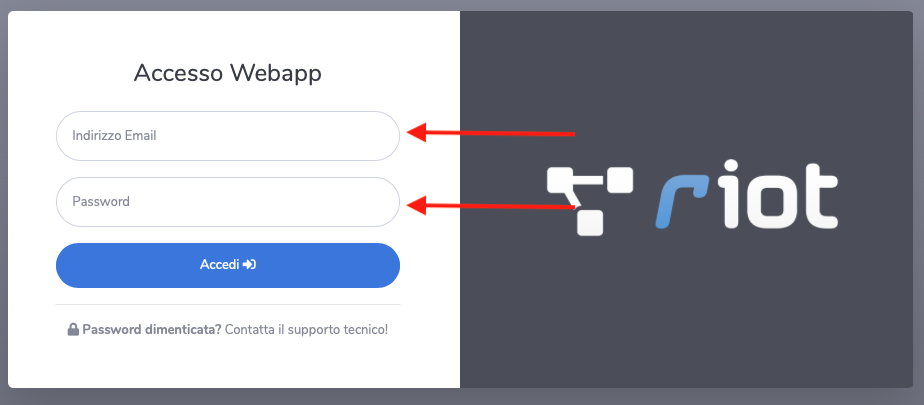
\includegraphics[scale=0.450]{res/images/membro/login.png}
		\caption{Login web app}
	\end{figure}

\newpage \subsection{1a. Accesso alla web app con TFA}
	
	\begin{itemize}
		\item \href{https://www.youtube.com/watch?v=PjySMOLCtMA&list=PLPKYjnuIh1FA3b3jn_bwY_ztYzaFn2mIT&index=2}{Visualizza il video tutorial su YouTube} 
	\end{itemize}
	Per eseguire il login alla webapp con un’autenticazione a due fattori, è necessario disporre di email, password e di un account Telegram registrato e abilitato dalle impostazioni.
	Nella schermata di login, una volta inserita l'email e la password, verrà inviato un codice numerico di 6 cifre sulla chat Telegram del Bot. 
	\begin{figure}[H]
		\centering
		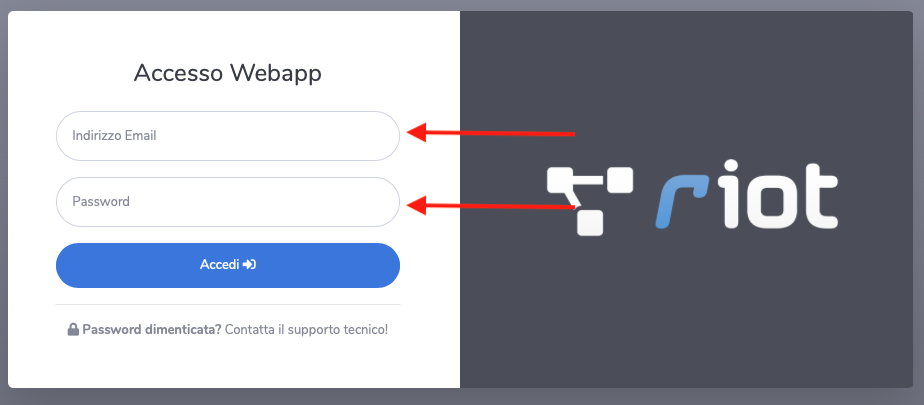
\includegraphics[scale=0.450]{res/images/membro/login.png}
		\caption{Login web app}
	\end{figure}
	\begin{figure}[H]
		\centering
		
\includegraphics[scale=0.600]{res/images/membro/tokenTFA.png}
		\caption{Codice di autenticazione su Telegram}
	\end{figure}
	Il codice sarà valido per 5 minuti. Una volta inserito il codice, si aprirà la dashboard e si sarà completato l'accesso al sito.
	\begin{figure}[H]
		\centering
		
\includegraphics[scale=0.600]{res/images/membro/loginTFA.png}
		\caption{Login con autenticazione a due fattori}
	\end{figure}


\newpage \subsection{1b. Visualizzazione dashboard e supporto tecnico}
	

	\begin{itemize}
		\item \href{https://www.youtube.com/watch?v=PjySMOLCtMA&list=PLPKYjnuIh1FA3b3jn_bwY_ztYzaFn2mIT&index=3}{Visualizza il video tutorial su YouTube} 
	\end{itemize}
	Una volta eseguito il login, è possibile visualizzare la dashboard con le proprie informazioni account, le statistiche del sito e le relative informazioni di supporto tecnico sulla destra.

	\begin{figure}[H]
		\centering
		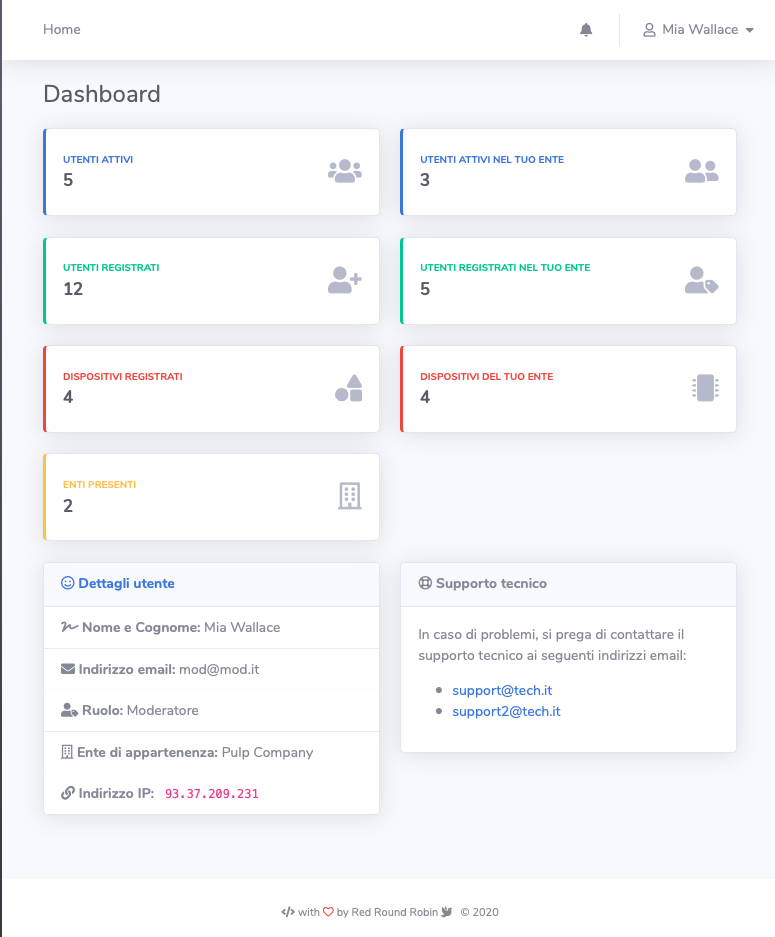
\includegraphics[scale=0.600]{res/images/membro/dashboard.png}
		\caption{Dashboard}
	\end{figure}

\newpage \subsection{2. Impostazioni account}

	\begin{itemize}
		\item \href{https://www.youtube.com/watch?v=PjySMOLCtMA&list=PLPKYjnuIh1FA3b3jn_bwY_ztYzaFn2mIT&index=4}{Visualizza il video tutorial su YouTube} 
	\end{itemize}
	Dalla dashboard è possibile entrare nelle impostazioni dalla sidebar o dal menù utente in alto a destra.
	\begin{figure}[H]
		\centering
		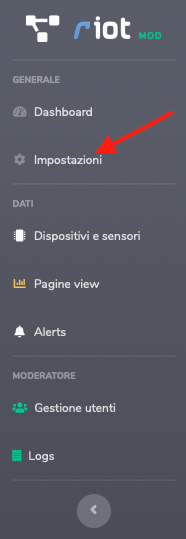
\includegraphics[scale=0.600]{res/images/membro/menuImp.png}
		\caption{Menu impostazioni}
	\end{figure}
	\begin{figure}[H]
		\centering
		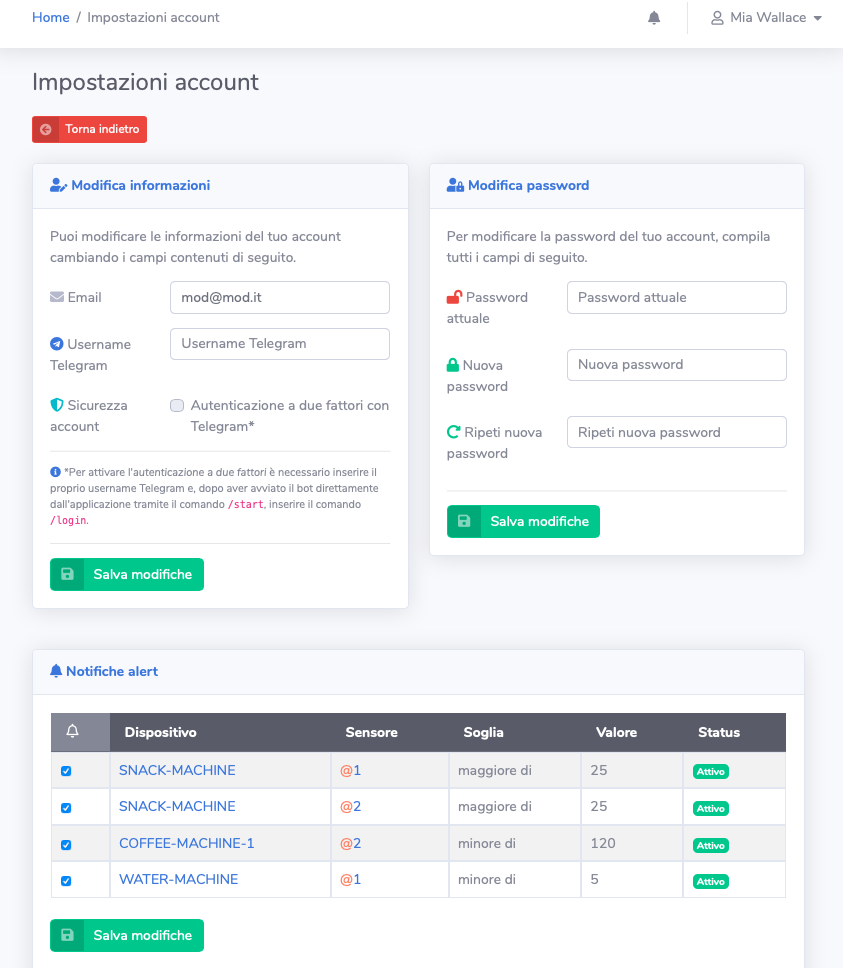
\includegraphics[scale=0.600]{res/images/membro/impostazioni.png}
		\caption{Impostazioni account}
	\end{figure}
	Da questa sezione è possibile modificare le proprie informazioni, la propria password e le notifiche alerts abilitati alla ricezione tramite il bot di Telegram.
	Le informazioni account modificabili sono la propria email e il proprio utente Telegram. Sempre da qui, è possibile abilitare l’autenticazione a due fattori, una volta registrato il proprio account con il bot Telegram.


	\subsubsection{Modifica email e Username Telegram - 0:15}

		\begin{figure}[H]
		\centering
		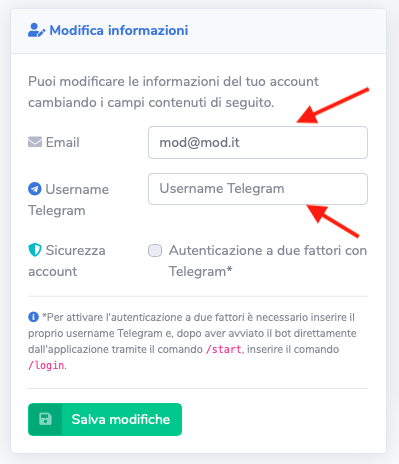
\includegraphics[scale=0.600]{res/images/membro/modUsername.png}
		\caption{Modifica username Telegram e email}
	\end{figure}
	Per modificare la propria email o lo username Telegram è sufficiente entrare nella sezione delle impostazioni e modificare i campi email o username Telegram.
	Infine è necessario premere sul bottone \textit{salva modifiche} per rendere le modifiche effettuate permanenti.

	\subsubsection{Modifica password - 0:36}

		\begin{figure}[H]
		\centering
		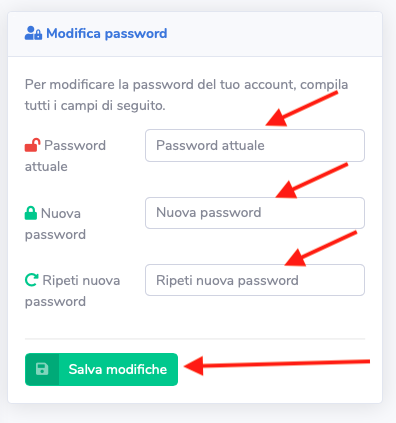
\includegraphics[scale=0.600]{res/images/membro/modPassword.png}
		\caption{Modifica password}
	\end{figure}
	Per la modifica password, è necessario inserire la password attuale e quella nuova purché rispetti il limite minimo di 6 caratteri.
	Infine è necessario ripetere la nuova password inserita e premere sul bottone \textit{salva modifiche}.

	\subsubsection{Attivazione e disattivazione alert - 0:47}

		\begin{figure}[H]
		\centering
		\includegraphics[scale=0.600]{res/images/membro/attDisattAlert.png}
		\caption{Attivazione e disattivazione alert}
	\end{figure}
	Una volta entrati nella sezione impostazioni, scorrendo verso il basso si trova una lista con tutti gli alert abilitati per il proprio ente. Cliccando sul checkbox corrispondente all'alert prescelto è possibile attivarlo o disattivarlo. Per rendere permanenti le modifiche è necessario premere sul bottone \textit{salva modifiche} posto in basso.
	

	\subsubsection{Configurazione Telegram}
		Per usufruire delle funzionalità di alert è necessario scaricare l'applicazione Telegram dallo store sul proprio dispositivo.
		Dopo aver avviato l'applicazione è necessario entrare nelle impostazioni cliccando prima sul menù ad hamburger in altro a sinistra sullo schermo.
		\begin{figure}[H]
			\centering
			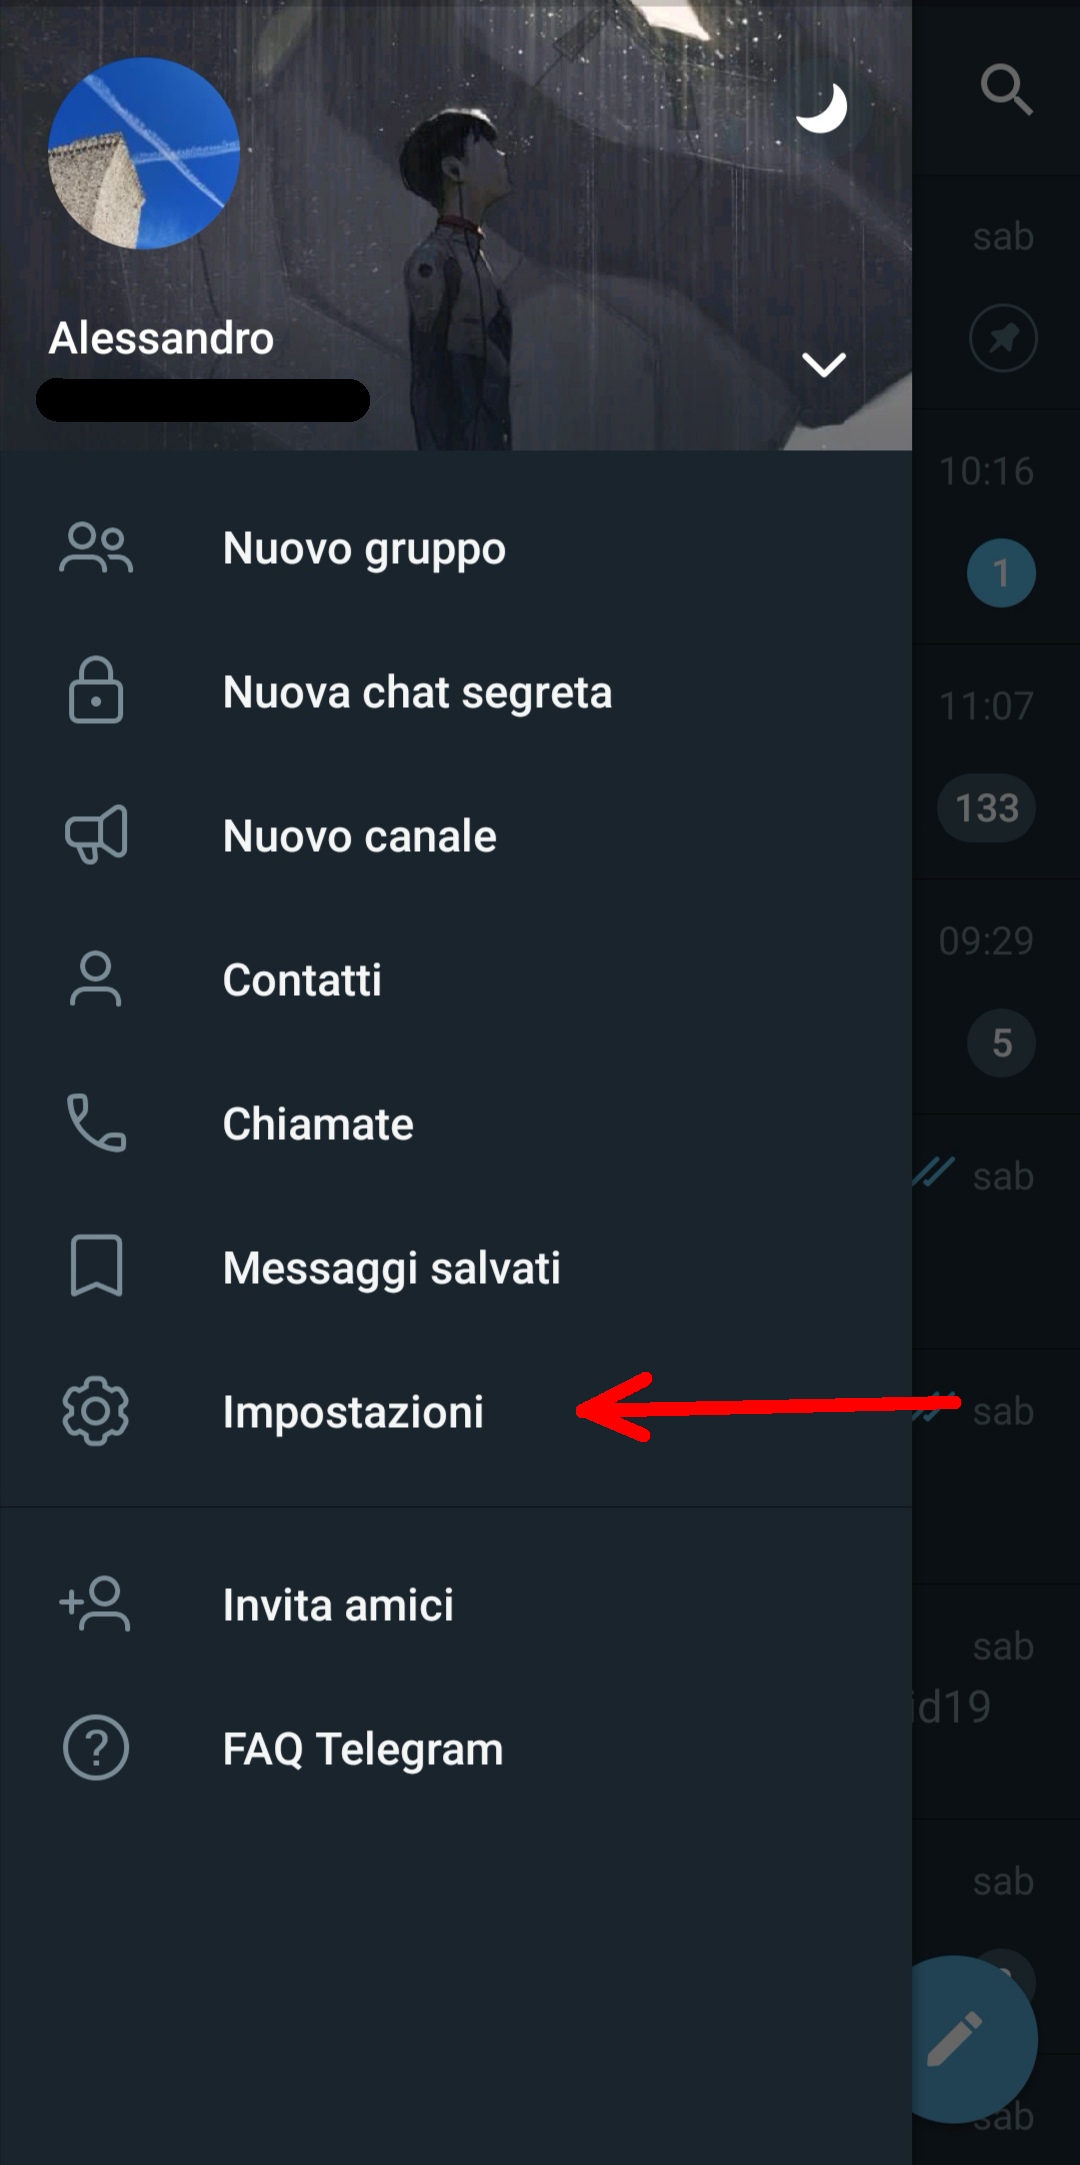
\includegraphics[scale=0.150]{res/images/telegram1.jpg}
			\caption{Come entrare nella sezione impostazioni su Telegram}
			\label{Screenshot1}
		\end{figure}
		\newpage
		In seguito è necessario cliccare nel punto indicato dalla freccia per poter inserire e/o modificare il proprio username
		\begin{figure}[H]
			\centering
			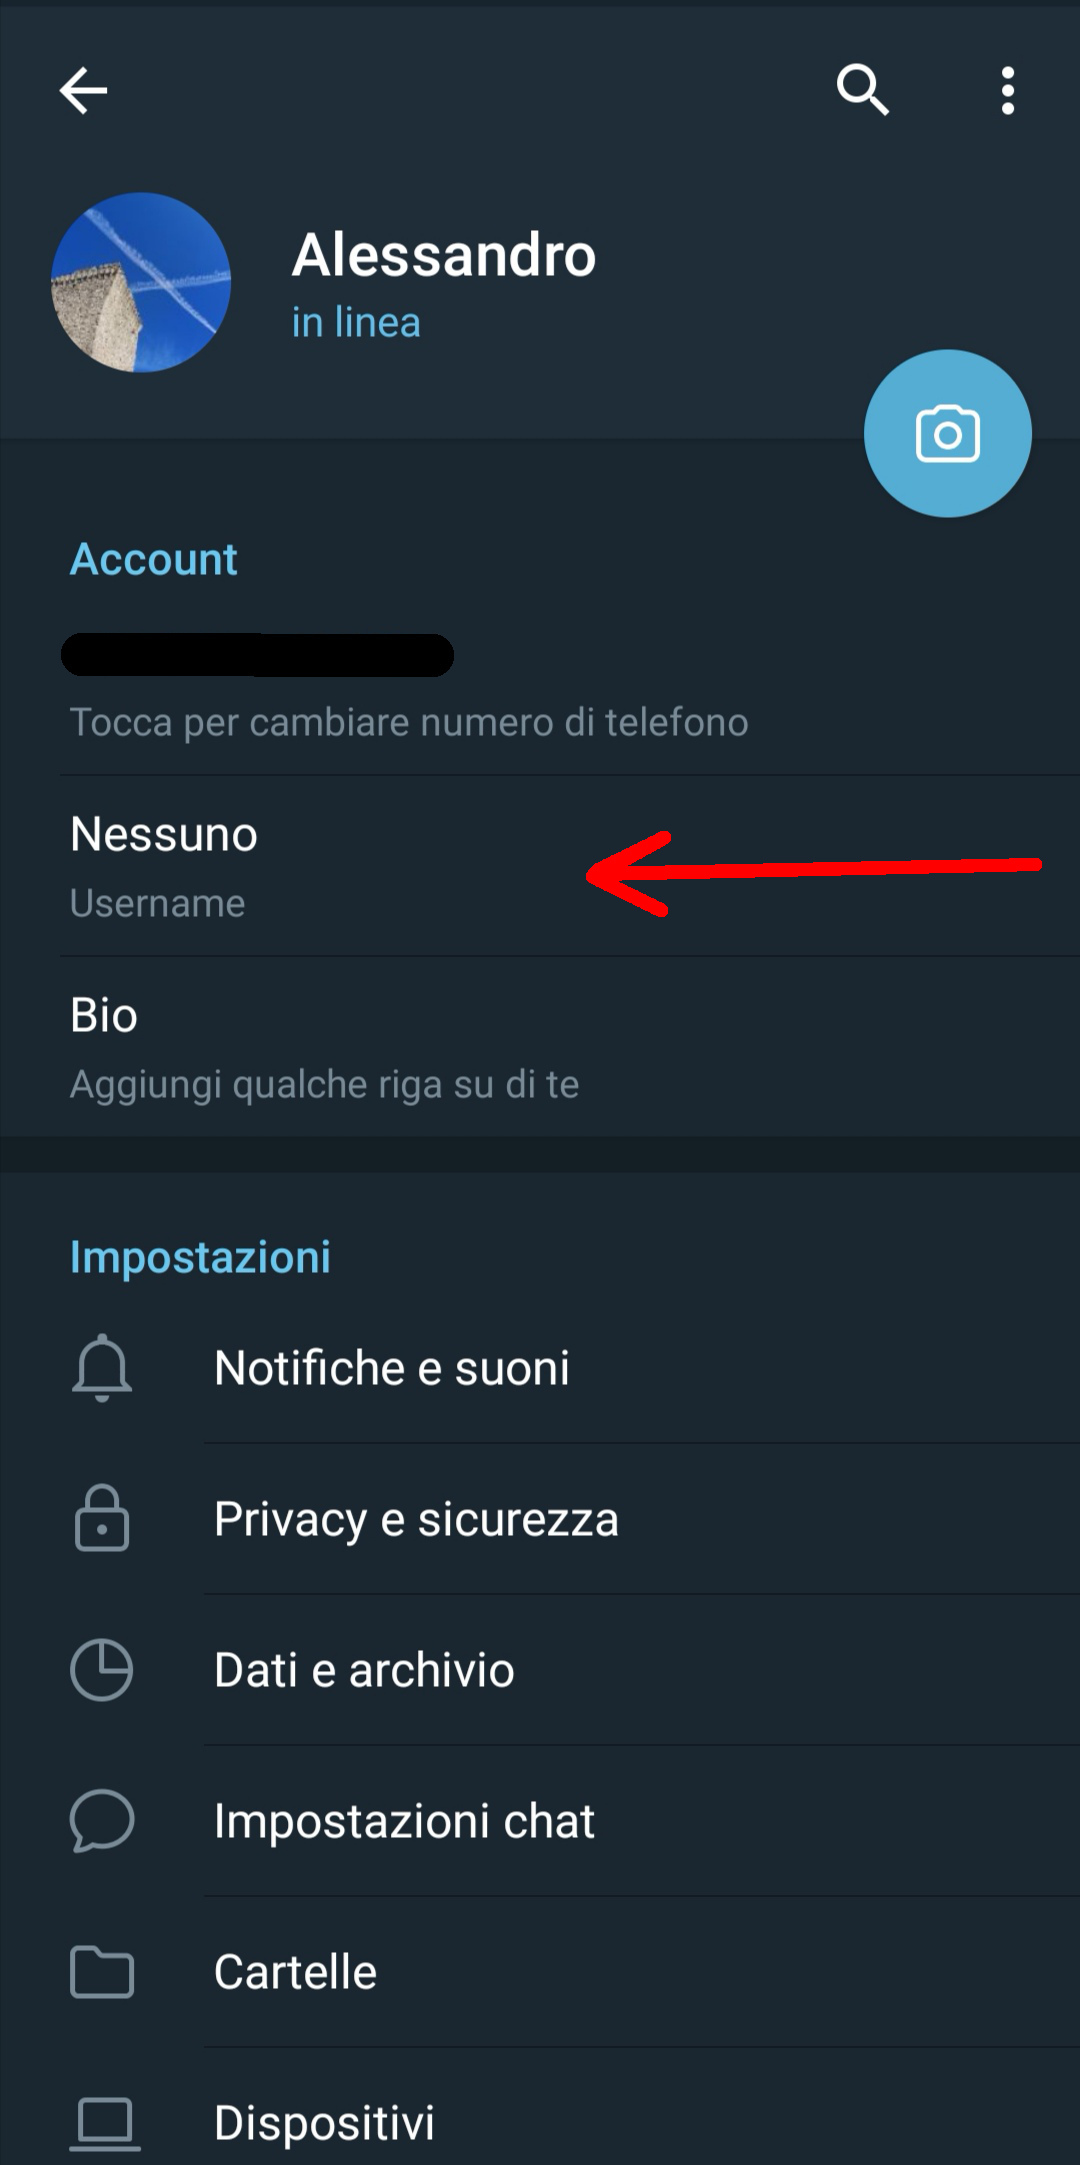
\includegraphics[scale=0.110]{res/images/telegram2.jpg}
			\caption{Come inserire uno username su Telegram}
			\label{Screenshot2}
		\end{figure}
		Infine è necessario inserire il nome nel campo indicato prestando attenzione ad inserire almeno 5 caratteri e salvare cliccando la spunta in alto a destra.
		\begin{figure}[H]
			\centering
			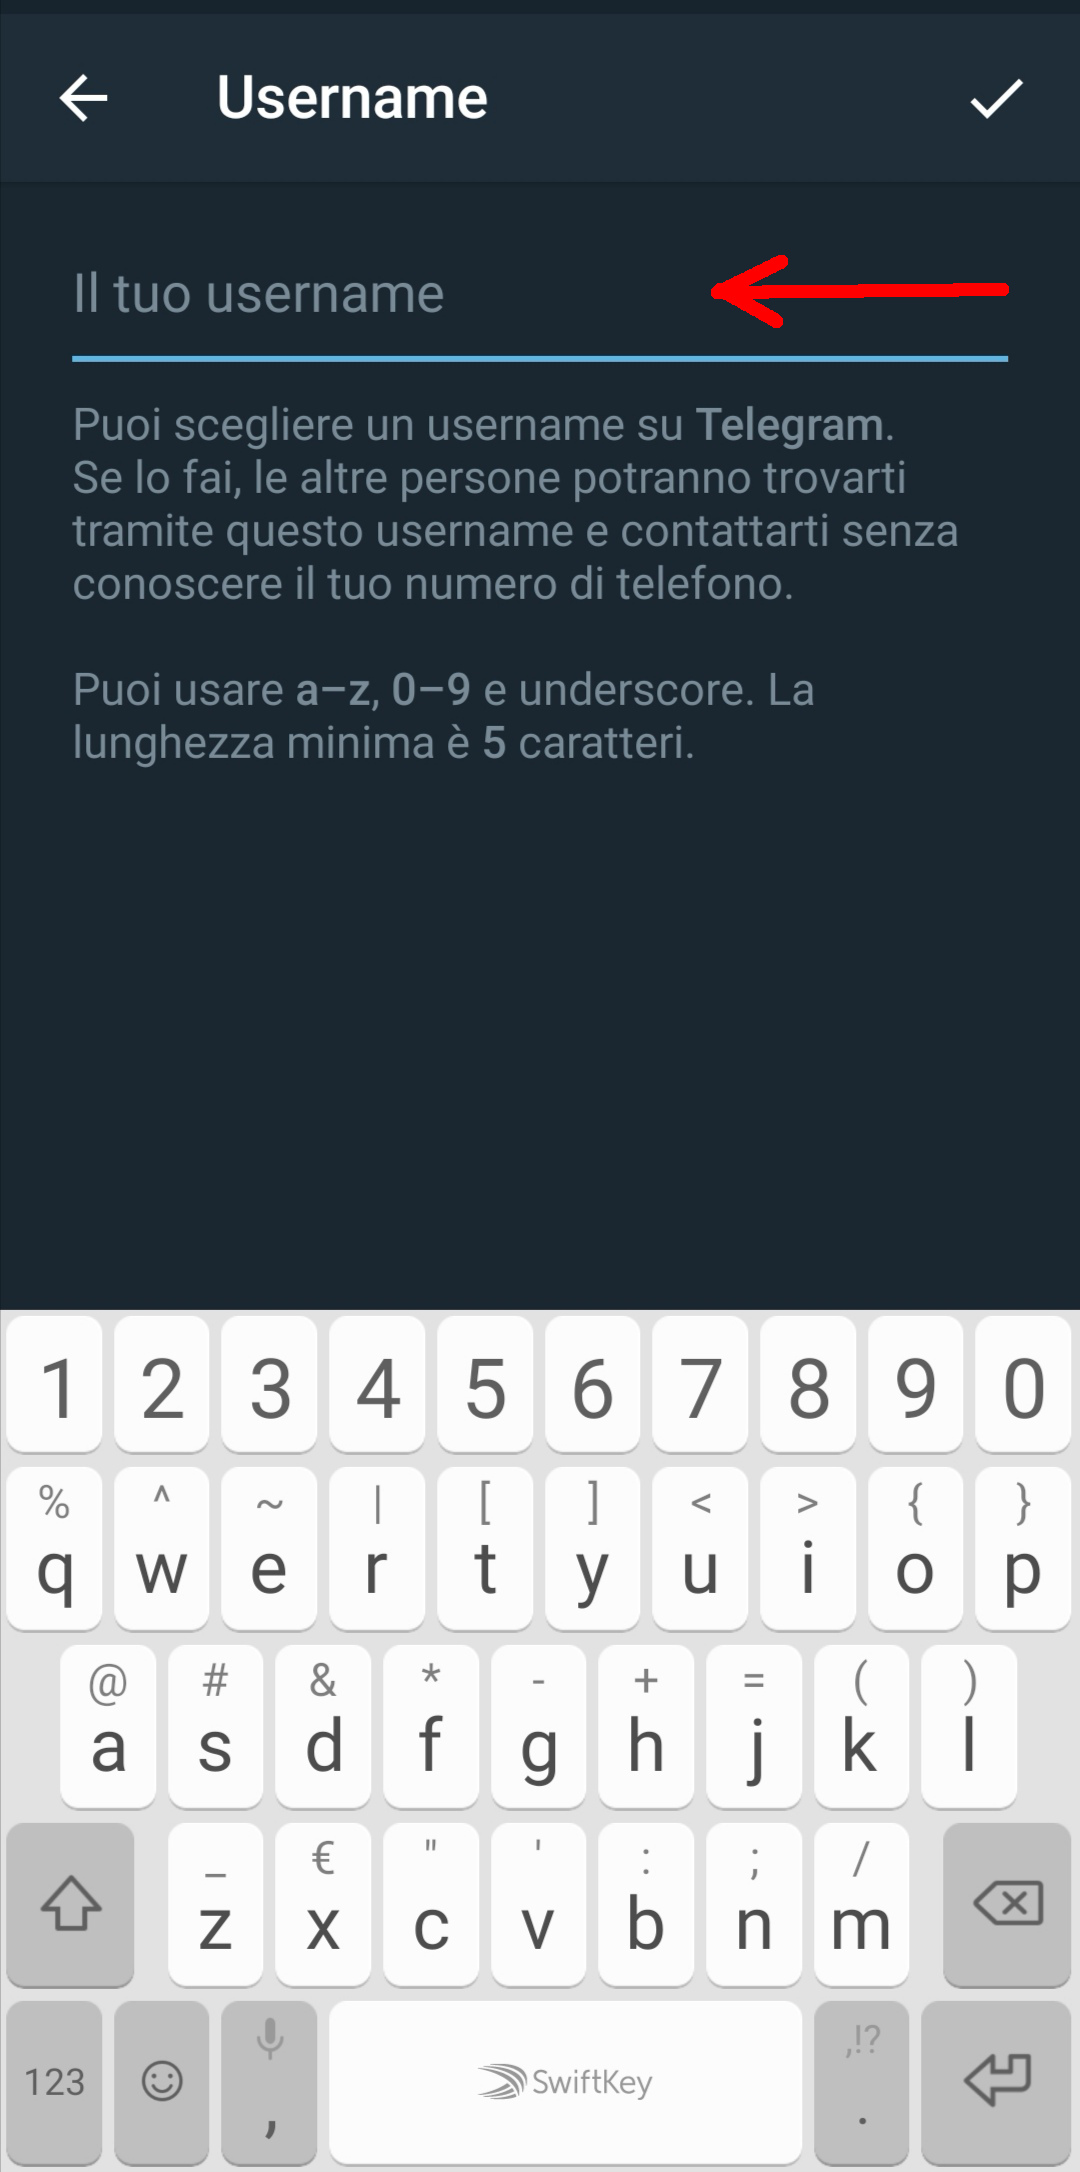
\includegraphics[scale=0.110]{res/images/telegram3.jpg}
			\caption{Come salvare lo username inserito su Telegram}
			\label{Screenshot3}
		\end{figure}

\newpage \subsection{2a. Abilitazione notifiche alert e TFA}

	\begin{itemize}
		\item \href{https://www.youtube.com/watch?v=PjySMOLCtMA&list=PLPKYjnuIh1FA3b3jn_bwY_ztYzaFn2mIT&index=5}{Visualizza il video tutorial su YouTube} 
	\end{itemize}

	\subsubsection{Modifica username Telegram su WebApp - 0:11}

		\begin{figure}[H]
		\centering
		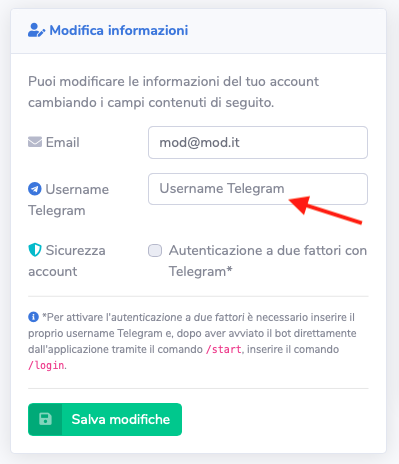
\includegraphics[scale=0.600]{res/images/membro/modUsername1.png}
		\caption{modifica username Telegram}
	\end{figure}
	\begin{figure}[H]
		\centering
		
\includegraphics[scale=0.600]{res/images/membro/modUsTelegram.png}
		\caption{modifica username Telegram dettaglio}
	\end{figure}
	Da Modifica informazioni all'interno della sezione impostazioni è possibile inserire il proprio nome account Telegram. Il nome Telegram è possibile recuperarlo dal proprio profilo Telegram ed è segnato con una chiocciola (@). Nel form è sufficiente riportare tale nome senza chiocciola.
	Una volta modificato, è necessario aprire il proprio telefono e aprire la chat con il nostro bot denominato RIoT.

	\subsubsection{Attivazione bot Telegram - 0:32}
	Dopo aver inserito il proprio username Telegram ed aver salvato le impostazioni, è necessario spostarsi all'interno dell'applicazione Telegram ed entrare nella chat con il bot RIoT che è possibile cercare tramite la barra di ricerca presente nell'applicazione.
	Premere quindi \textit{Avvia} in basso.

		\begin{figure}[H]
		\centering
		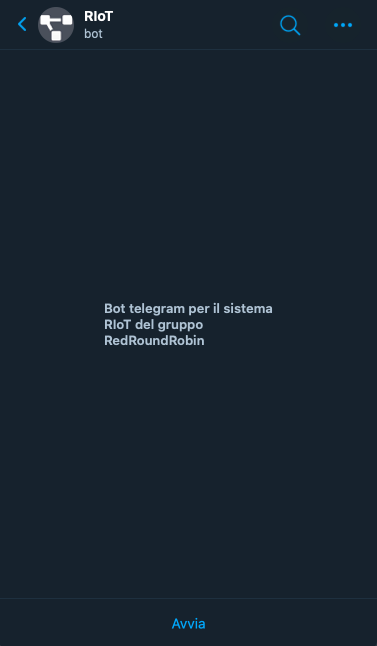
\includegraphics[scale=0.600]{res/images/membro/avvioBot.png}
		\caption{Avvio bot Telegram}
	\end{figure}
	\begin{figure}[H]
		\centering
		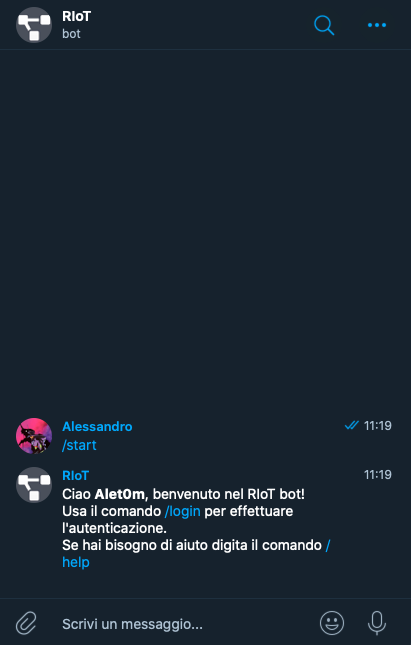
\includegraphics[scale=0.600]{res/images/membro/mexBenvenuto.png}
		\caption{Messaggio di benvenuto su Telegram}
	\end{figure}

		Questo ci mostrerà un messaggio di benvenuto.
		Successivamente digitare /login nella chat. Il bot controllerà il nostro nome utente e ci registrerà al sistema.

		\begin{figure}[H]
		\centering
		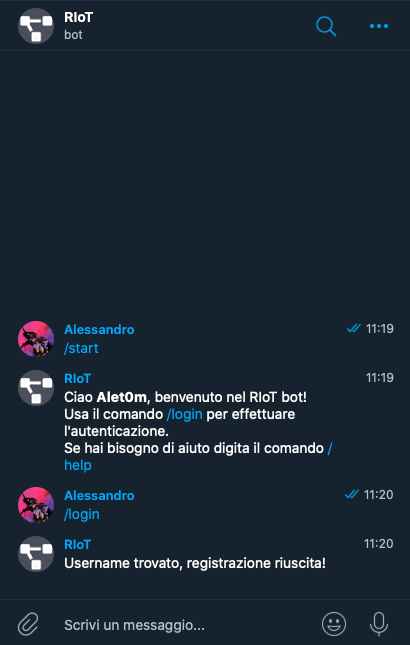
\includegraphics[scale=0.600]{res/images/membro/loginTelegram.png}
		\caption{Comando login su Telegram}
	\end{figure}
	A questo punto sarà possibile ricevere in automatico le notifiche alert segnate come attive nelle impostazioni.
 

	\subsubsection{Abilitazione TFA - 0:54}
	Prima di abilitare questa funzione è necessario aver completato la registrazione del proprio username Telegram seguendo la procedura alla sezione \textbf{Attivazione bot Telegram}.
	\begin{figure}[H]
		\centering
		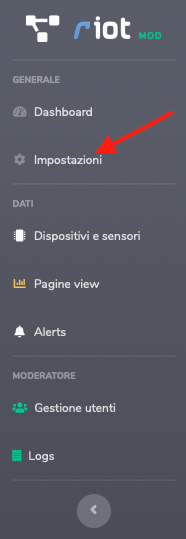
\includegraphics[scale=0.600]{res/images/membro/menuImp.png}
		\caption{Menu impostazioni}
	\end{figure}	
	Per abilitare l'autenticazione a due fattori (TFA) è necessario entrare nella sezione impostazioni del sito.
	\begin{figure}[H]
		\centering
		
\includegraphics[scale=0.600]{res/images/membro/TFAAbilitato.png}
		\caption{Abilitazione TFA}
	\end{figure}
	Attivata la spunta su quest'ultima, sarà sufficiente cliccare su salva modifiche e l'autenticazione a due fattori sarà abilitata.



\newpage \subsection{3. Alerts e impostazioni di notifica}

	\begin{itemize}
		\item \href{https://www.youtube.com/watch?v=PjySMOLCtMA&list=PLPKYjnuIh1FA3b3jn_bwY_ztYzaFn2mIT&index=6}{Visualizza il video tutorial su YouTube} 
	\end{itemize}

	\subsubsection{Visualizzazione lista alert attivi - 0:05}
	Una volta entrati nella sezione impostazioni, scorrendo verso il basso si trova una lista con tutti gli alert abilitati per il proprio ente.
		\begin{figure}[H]
		\centering
		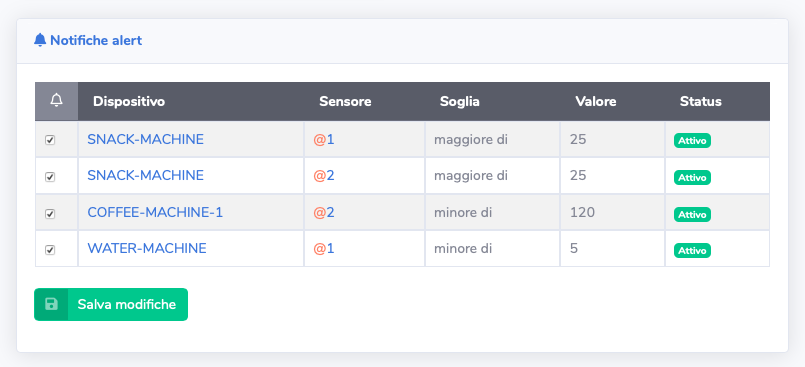
\includegraphics[scale=0.600]{res/images/membro/listaAlert.png}
		\caption{Lista alert}
	\end{figure}

	\subsubsection{Modifica preferenze di ricezione alert - 0:38}
		Per modificare le proprie preferenze di ricezione alerts, è sufficiente procedere nelle proprie impostazioni e muoversi in basso nella pagina.
		\begin{figure}[H]
		\centering
		\includegraphics[scale=0.600]{res/images/membro/attDisattAlert.png}
		\caption{Modifica preferenze di ricezione degli alert}
	\end{figure}
	Una volta qui, è sufficiente spuntare gli alerts che si vogliono abilitare. Gli alerts abilitati verranno notificati tramite Telegram quando avverrà il superamento della soglia impostata per un dato sensore.


\newpage \subsection{4 . Pagine view}
	
	\begin{itemize}
		\item \href{https://www.youtube.com/watch?v=PjySMOLCtMA&list=PLPKYjnuIh1FA3b3jn_bwY_ztYzaFn2mIT&index=7}{Visualizza il video tutorial su YouTube} 
	\end{itemize}

	\begin{figure}[H]
		\centering
		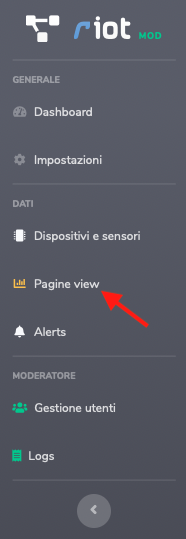
\includegraphics[scale=0.600]{res/images/membro/menuView.png}
		\caption{Menu view}
	\end{figure}
	Dalla sidebar a sinistra è possibile raggiungere la sezione pagine view.
	Questa sezione permette di creare delle pagine personalizzate in cui inserire una serie di grafici di cui si vuole eseguire il monitoraggio in tempo reale da un'unica finestra.
	\begin{figure}[H]
		\centering
		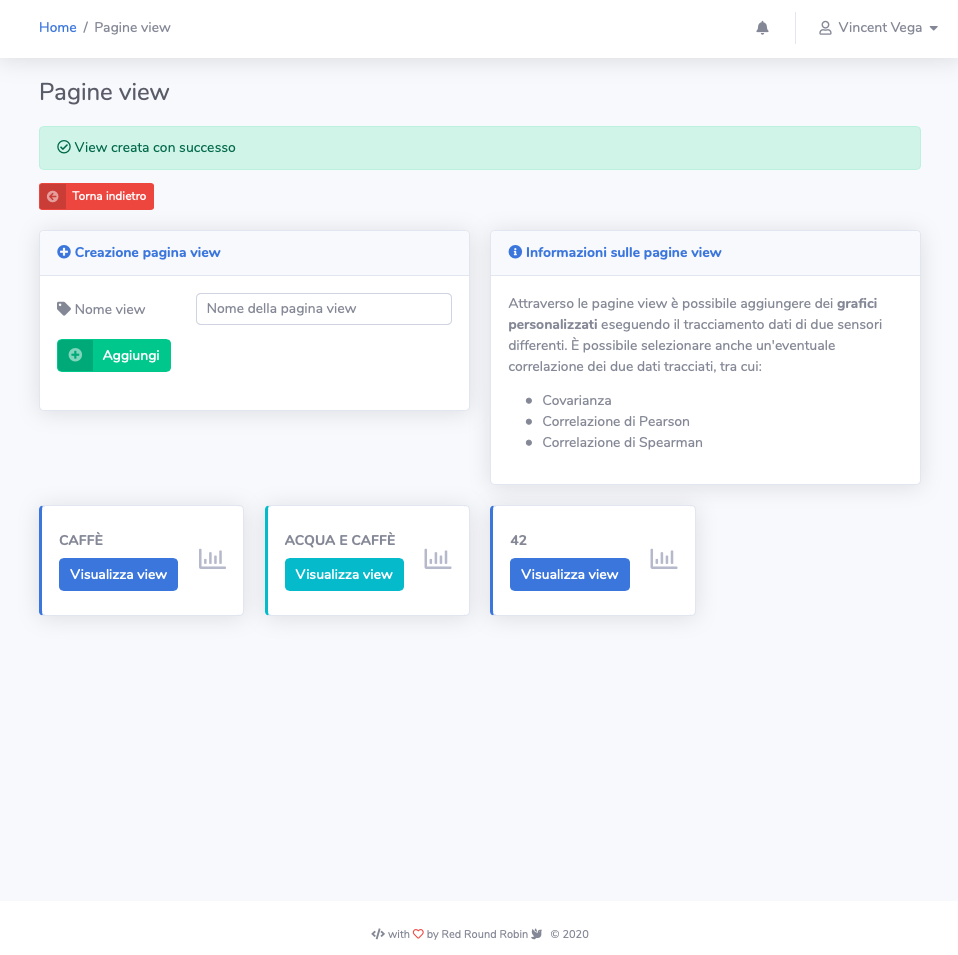
\includegraphics[scale=0.400]{res/images/membro/view.png}
		\caption{Sezione view}
	\end{figure}

	\subsubsection{Creazione nuova view - 0:08}
	\begin{figure}[H]
		\centering
		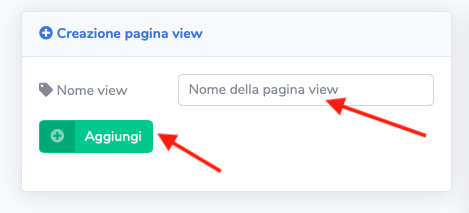
\includegraphics[scale=0.600]{res/images/membro/creazView.png}
		\caption{Creazione view}
	\end{figure}
	Per creare una view è sufficiente entrare nella sezione View e, dopo aver inserito il nome prescelto all'interno del campo, premere sul bottone aggiungi.

	\subsubsection{Creazione nuovo grafico - 0:33}
		Per creare un grafico in una view è necessario disporre di almeno una view.
		\begin{figure}[H]
		\centering
		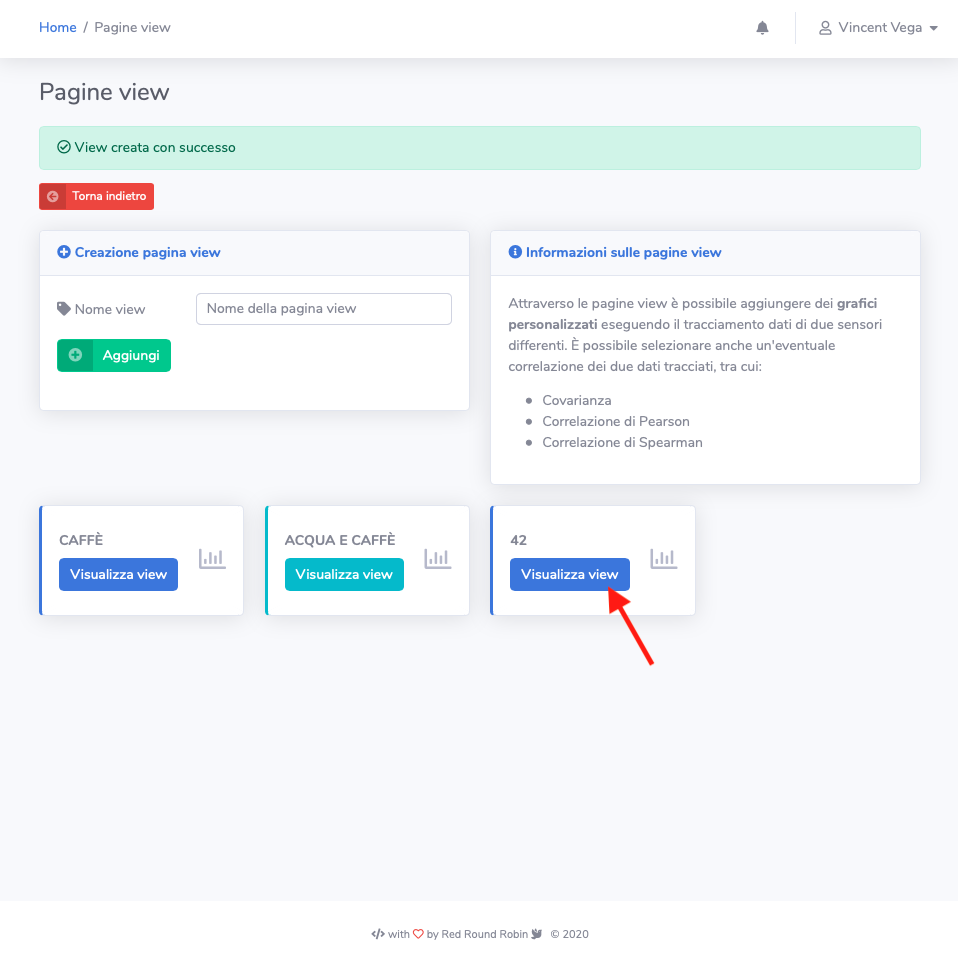
\includegraphics[scale=0.400]{res/images/membro/selView.png}
		\caption{Selezione e visualizzazione lista view}
	\end{figure}
		Dalla sezione View è necessario cliccare sul bottone \textit{visualizza view} della view a cui si vuole aggiungere un grafico.
		\begin{figure}[H]
		\centering
		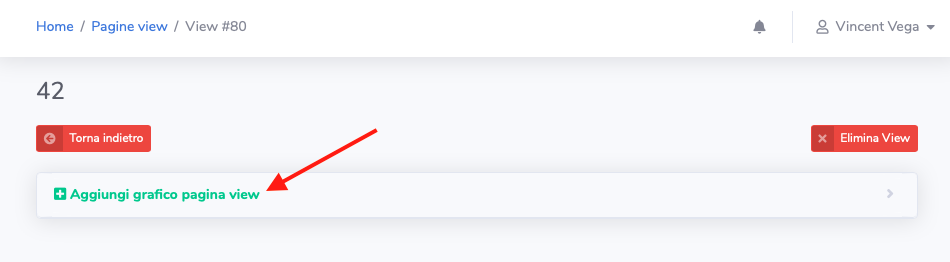
\includegraphics[scale=0.450]{res/images/membro/clicAggGrafico.png}
		\caption{Aggiunta grafico pagina view}
	\end{figure}
		In seguito è necessario cliccare su \textit{aggiungi} grafico pagina view. 
		\begin{figure}[H]
		\centering
		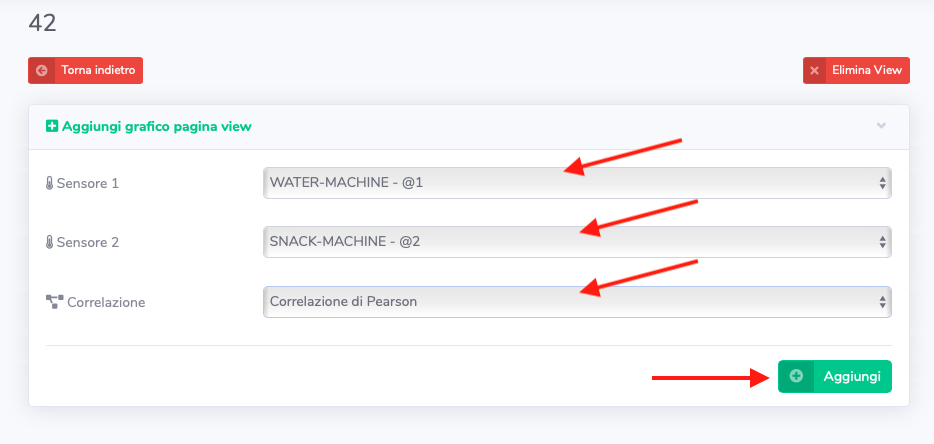
\includegraphics[scale=0.450]{res/images/membro/insDatiGrafico.png}
		\caption{Inserimento dati grafico pagina view}
	\end{figure}
		Questo aprirà un form in cui è possibile inserire i due sensori e l'eventuale correlazione da mostrare nel grafico. Una volta compilati i campi è sufficiente cliccare su \textit{aggiungi} e il grafico verrà inserito all'interno della view.

	\subsubsection{Eliminazione grafico - 1:17}
		Per eliminare un grafico è necessario entrare nella view a cui appartiene il grafico da rimuovere. 
		\begin{figure}[H]
		\centering
		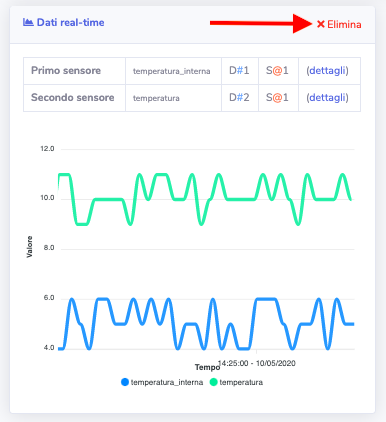
\includegraphics[scale=0.700]{res/images/membro/eliminazGrafico.png}
		\caption{Eliminazione grafico}
		\end{figure}
		Infine, è sufficiente cliccare su \textit{elimina} posto nell'angolo in alto a destra del grafico (prestare attenzione a non cliccare sul bottone \textit{elimina view} in alto a destra nella pagina).

	\subsubsection{Eliminazione view - 2:00}
		\begin{figure}[H]
		\centering
		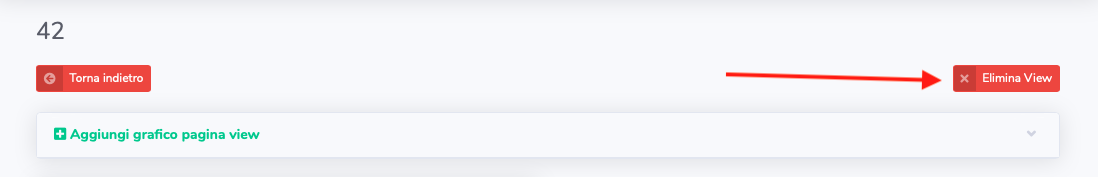
\includegraphics[scale=0.450]{res/images/membro/eliminazView.png}
		\caption{Eliminazione view}
		\end{figure}
		Per eliminare una view è sufficiente entrare all'interno della view che si intende eliminare e cliccare sul bottone \textit{elimina view} posto in altro a destra nella pagina.
	

\newpage \subsection{5. Dispositivi e sensori}
	
	\begin{itemize}
		\item \href{https://www.youtube.com/watch?v=PjySMOLCtMA&list=PLPKYjnuIh1FA3b3jn_bwY_ztYzaFn2mIT&index=8}{Visualizza il video tutorial su YouTube} 
	\end{itemize}

	\subsubsection{Visualizzazione lista dispositivi - 0:05}
		\begin{figure}[H]
		\centering
		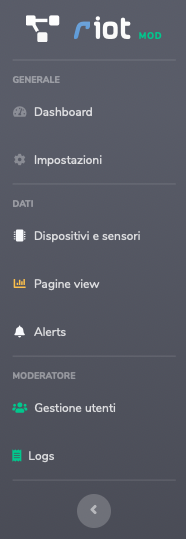
\includegraphics[scale=0.600]{res/images/membro/menuDisp.png}
		\caption{Menu dispositivi e sensori}
		\end{figure}
		Dalla sidebar è possibile raggiungere la sezione dispositivi e sensori a sinistra. 
		\begin{figure}[H]
		\centering
		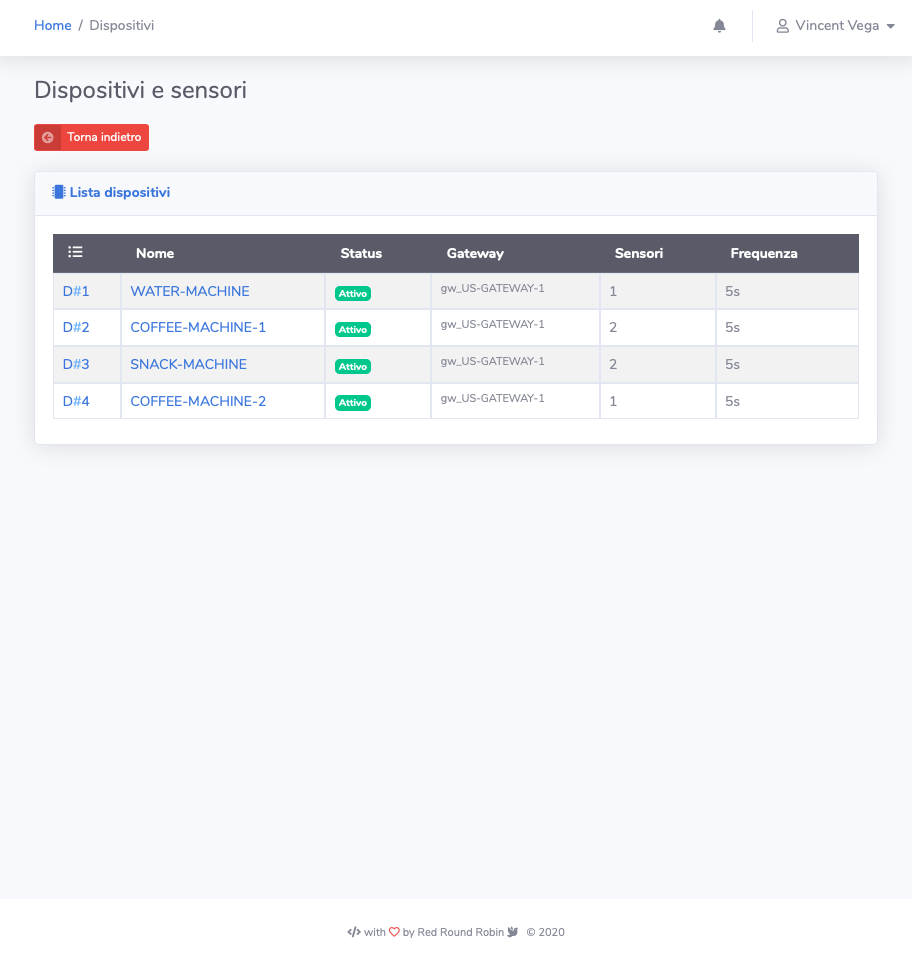
\includegraphics[scale=0.450]{res/images/membro/visDispositivi.png}
		\caption{Visualizzazione dispositivi}
		\end{figure}
		Questa sezione permette di visualizzare tutti i dispositivi abilitati del proprio ente e permette di visionare nel dettaglio le informazioni di un dispositivo.
		In particolare, lo status, il gateway di appartenenza, il numero di sensori e la frequenza di ricezione dati. 


	\subsubsection{ID logico e ID reale - 0:20}
		\begin{figure}[H]
		\centering
		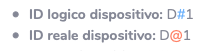
\includegraphics[scale=0.700]{res/images/membro/IDLogicoIDReale.png}
		\caption{ID logico e ID reale}
		\end{figure}
		In giro per la web app, inoltre, si troveranno spesso questi due simboli, cancelletto (\#) e chiocciola (@). Il primo identifica che l'id riportato è un ID logico, utilizzato dai tecnici del database, mentre il secondo è l'id reale del dispositivo, utilizzato dagli amministratori del sistema, per identificare l'id effettivo del dispositivo che il gateway deve contattare.

	\subsubsection{Visualizzazione sensori di un dispositivo - 0:40}
		Per visualizzare la lista dei sensori di un dispositivo è necessario entrare nella sezione di gestione dei dispositivi e cliccare sul nome o ID del dispositivo prescelto.
		\begin{figure}[H]
		\centering
		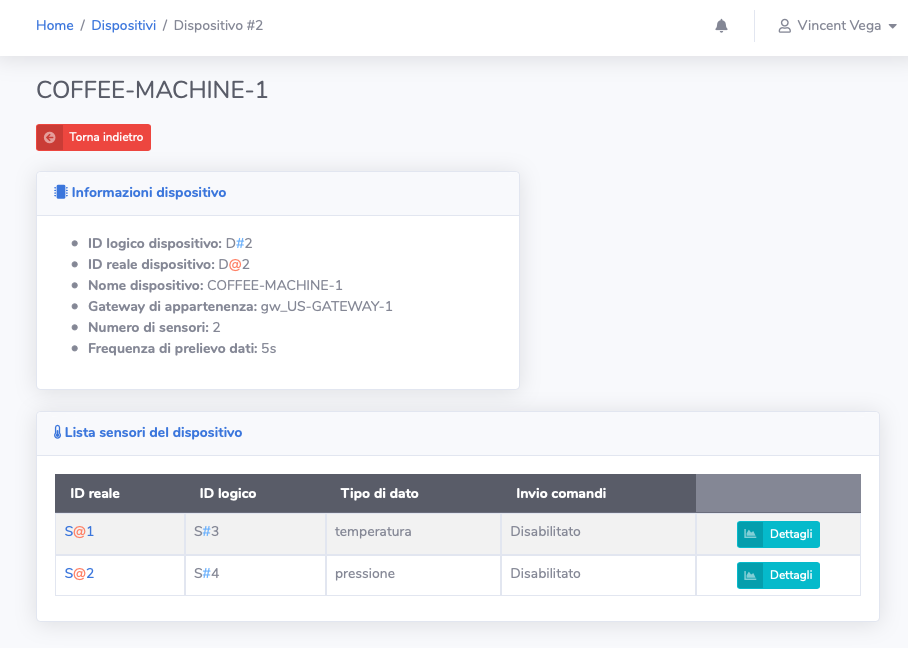
\includegraphics[scale=0.450]{res/images/membro/visSensori.png}
		\caption{Visualizzazione sensori di un dispositivo}
		\end{figure}
		Questo provocherà l'apertura di una pagina in cui vengono visualizzate sia le informazioni de dispositivo che, più in basso la lista con tutti i suoi sensori.

	\subsubsection{Visualizzazione grafico di un sensore - 1:00}
		Per visualizzare il grafico di un sensore è necessario entrare all'interno della pagina di dettaglio di un dispositivo (seguire sezione \textbf{Visualizzazione sensori di un dispositivo}) e cliccare sul bottone Dettagli associato al dispositivo di cui si vuole vedere il grafico.
		\begin{figure}[H]
		\centering
		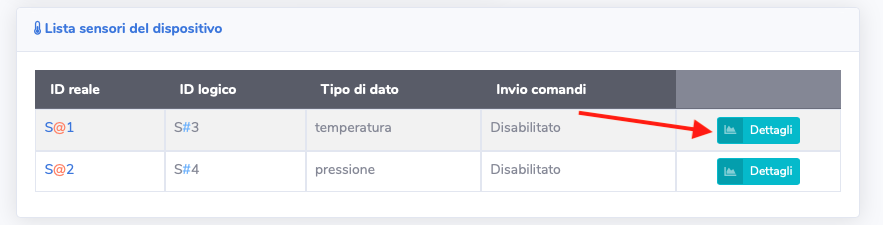
\includegraphics[scale=0.500]{res/images/membro/clicGraficoSens.png}
		\caption{Bottone per visualizzare il grafico di un sensore}
		\end{figure}
		\begin{figure}[H]
		\centering
		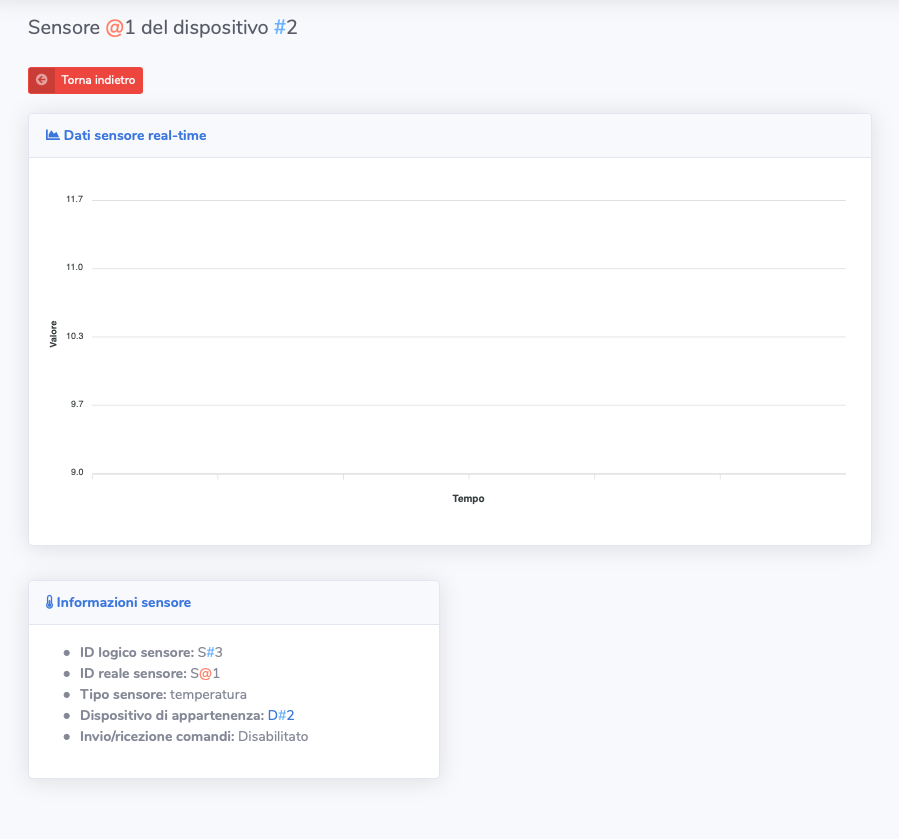
\includegraphics[scale=0.650]{res/images/membro/graficoSens.png}
		\caption{Visualizzazione grafico di un sensore}
		\end{figure}
		

